\documentclass{article}
\usepackage[utf8]{inputenc}
\usepackage[fontset=ubuntu]{ctex}
\usepackage{ctex}
\usepackage{cite}
\usepackage{siunitx}
\usepackage{enumerate}
\usepackage{amsfonts}
\usepackage{amsmath}
\usepackage{physics}
\usepackage{graphicx}
\usepackage{subfigure}
\usepackage{authblk}
\usepackage{float}
\usepackage{listings}
\usepackage{color,xcolor}
\numberwithin{equation}{subsection}

\lstset{
    basicstyle          =   \sffamily,          % 基本代码风格
    keywordstyle        =   \bfseries,          % 关键字风格
    commentstyle        =   \rmfamily\itshape,  % 注释的风格,斜体
    stringstyle         =   \ttfamily,  % 字符串风格
    flexiblecolumns,                % 别问为什么,加上这个
    numbers             =   left,   % 行号的位置在左边
    showspaces          =   false,  % 是否显示空格,显示了有点乱,所以不现实了
    numberstyle         =   \zihao{-5}\ttfamily,    % 行号的样式,小五号,tt等宽字体
    showstringspaces    =   false,
    captionpos          =   t,      % 这段代码的名字所呈现的位置,t指的是top上面
    frame               =   lrtb,   % 显示边框
}

\lstdefinestyle{Python}{
    language        =   Python, % 语言选Python
    basicstyle      =   \zihao{-5}\ttfamily,
    numberstyle     =   \zihao{-5}\ttfamily,
    keywordstyle    =   \color{blue},
    keywordstyle    =   [2] \color{teal},
    stringstyle     =   \color{magenta},
    commentstyle    =   \color{red}\ttfamily,
    breaklines      =   true,   % 自动换行,建议不要写太长的行
    columns         =   fixed,  % 如果不加这一句,字间距就不固定,很丑,必须加
    basewidth       =   0.5em,
}

\newcommand*{\dif}{\mathop{}\!\mathrm{d}}
\renewcommand{\abstractname}{\large 摘要\\}
\providecommand{\keywords}[1]{\textbf{\textit{关键词:}} #1}

\title{计算物理大作业-PDE有限差分法的稳定性分析}
\author{}
\begin{document}

\maketitle
\begin{flushleft}
\large
作者: 吴远清\\
学号: 2018300001031\\
邮箱: yuanqingwu@whu.edu.cn\\
学院: 武汉大学,弘毅学堂\\
电话: 17352918073
\end{flushleft}
\clearpage
\begin{abstract}
    有限差分法是对PDE进行数值求解的一种重要方法,也是本课程中主要学习的方法.但是,本课程对于有限差分法的数值稳定性没有作较为详细而严谨的介绍.本文以一维扩散方程为例,介绍了对有限差分法稳定性分析常用的Von Neumann分析法,分别对于显示差分和隐式差分,求解了参数与数值稳定性间的关系,并做了验证.
\end{abstract}
\begin{keywords}
一维扩散方程,数值方法,lax等价定理,Von Neumann稳定性分析 
\end{keywords}
\section{研究背景}
由于偏微分方程解析求解面临着极大的困难,PDE的数值解法就显得尤为重要.其中,有限差分法是最简单,应用也最广泛的方法.本课程也主要教授有限差分法相关的内容.教材中指出,有些算法的数值稳定性存在问题\cite{giordano_computational_2006}.但并未给出详细的讨论和证明.事实上,对于不同的算法,其数值稳定性可能依赖于离散化网格的参数,也可能对于几乎所有参数都非常稳定或者非常不稳定\cite{thijssen_computational_2007}.这种差异和对参数的依赖使得对有限差分法的稳定性的研究具有非常重要的意义.我接下来将介绍一种数学上严格的稳定性分析方法,并使用对同一问题的两种离散方式来说明算法稳定性对数值计算的重要性.
\section{理论基础}
首先,我需要指出,本文中介绍的分析方法只适用于部分偏微分方程.更准确的说,是满足\textbf{Lax–Richtmyer条件}的偏微分方程.Lax和Richtmyer证明了如下结论\cite{lax_survey_1956}:\\
\emph{对于一个良好的线性初始值问题的一致的有限差分法,当且仅当它是稳定的时候,该方法是收敛的.}\\
这个定理表明,对于一些PDE系统,系统的稳定性与收敛性是等价的.Lax-Richtmyer条件为,PDE是线性的,且与差分格式相容.事实上,对于我们课程内求解的绝大多数体系,Lax-Richtmyer条件均满足.在此条件的基础上,Von Neumann提出了一套可以分析差分格式稳定性的方法\cite{charney_numerical_1950}.大致流程如下:
\begin{enumerate}[(1)]
    \item 将数值解与真实解之差$\epsilon$做傅里叶变换.
    \item 计算每次迭代的误差涨幅$G = \epsilon^{n+1}/\epsilon^n$.
    \item 若$|G|\leq 1$,则该差分格式是稳定的,否则,该差分格式是不稳定的.
\end{enumerate}
这就是所谓的Von Neumann稳定性分析(也称傅里叶稳定性分析).下面,我将以经典的一维扩散方程为例,利用Von Neumann稳定性分析来计算两种不同的差分格式的稳定性差别.
\section{稳定性分析}
我在此研究一维扩散问题,方程可写为\cite{scherer_computational_2013}:
\begin{equation}
    \frac{\partial u}{\partial t} = \alpha \frac{\partial^2 u}{\partial t^2}
\end{equation}
其中$\alpha$为一常数($\alpha>0$).
\subsection{显式格式差分}
首先,最自然的,我们使用显示格式差分:
\begin{equation}
    \frac{u^{n+1}_j - u^n_j}{\Delta t} = \alpha\frac{u^n_{j+1}-2u^n_j + u^n_{j-1}}{(\Delta x)^2}
\end{equation}
重排,得到:
\begin{equation}
    u^{n+1}_j = u^n_j + \frac{\alpha \Delta t}{(\Delta x)^2}(u^n_{j+1}-2*u^n_j+u^n_{j-1})
\end{equation}
该差分格式的数值解$N^n_j$和体系的真实解$T^n_j$均满足方程(3.1.2),并且由于其是线性方程,误差$\epsilon^n_j = N^n_j - T^n_j$也满足此方程,代入得:
\begin{equation}
    \epsilon^{n+1}_j = \epsilon^n_j + \frac{\alpha \Delta t}{(\Delta x)^2}(\epsilon^n_{j+1}-2\epsilon^n_j+\epsilon^n_{j-1})
\end{equation}
对误差$\epsilon$做傅里叶展开,有:
\begin{equation}
    \epsilon(x,t) = \sum_{m=1}^{N_x}e^{at}e^{ik_m x}
\end{equation}
其中,$a$为常数,$k_m = \frac{\pi m}{L}$,$N_x$为差分格式的x网格数.并且,再次由线性性质可知:
\begin{equation}
    G = \frac{\epsilon(x,t+\Delta t)}{\epsilon(x,t)} = \frac{e^{a(t+\Delta t)e^{ik_m x}}}{e^{at}e^{ik_m x}} = e^{a\Delta t}
\end{equation}
回到(3.1.3):
\begin{equation}
    e^{a \Delta t}=1+\frac{\alpha \Delta t}{\Delta x^{2}}\left(e^{i k_{m} \Delta x}+e^{-i k_{m} \Delta x}-2\right)
\end{equation}
由Euler公式:
\begin{equation}
    \sin ^{2} \frac{k_{m} \Delta x}{2} = -\frac{1}{4}\left(e^{i k_{m} \Delta x}+e^{-i k_{m} \Delta x}-2\right)
\end{equation}
由此有:
\begin{equation}
    G = 1-\frac{4 \alpha \Delta t}{\Delta x^{2}} \sin ^{2}\left(k_{m} \Delta x / 2\right)
\end{equation}
若要差分格式稳定,即$|G|\leq 1$:
\begin{equation}
    \frac{\alpha \Delta t}{\Delta x^{2}} \leq \frac{1}{2}
\end{equation}
至此,我们通过Von Neumann方法,成功的讨论了一维扩散方程的显式格式差分的稳定性条件.可见,随着体系网格的缩小,时间步长也需要减小,以维持计算稳定,这符合我们的预期.\\
接下来,我们进行实际计算来测试方程(3.1.9)的结论是否正确,我们定义$\alpha\Delta t/(\Delta x)^2$为$\beta$,调节不同的$\Delta t$和$\Delta x$的值,来验证体系的稳定性,代码见附录(代码1).\\
首先,我们计算了两组不同的$\Delta x$和$\Delta t$下的一维扩散方程,但均保持$\beta = 0.5$,结果如下图(见图1,图2),可见,体系均能保持稳定.\\

\begin{figure}[H]
\centering
\subfigure[t=0]{
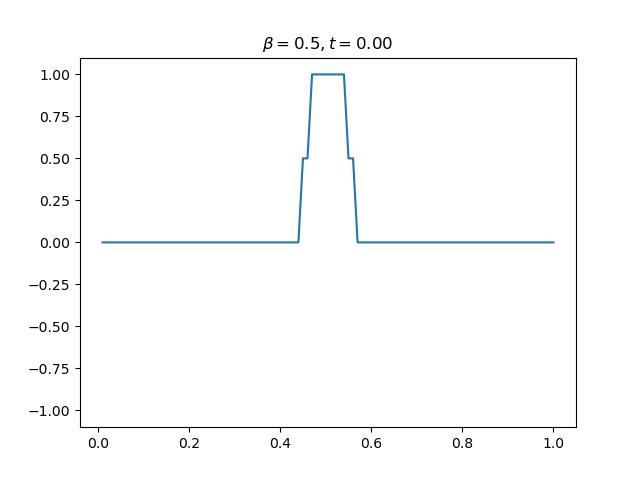
\includegraphics[width=5.5cm]{img/explicit/0.5-0.01/1.jpg}
%\caption{fig1}
}
\quad
\subfigure[t=0.01]{
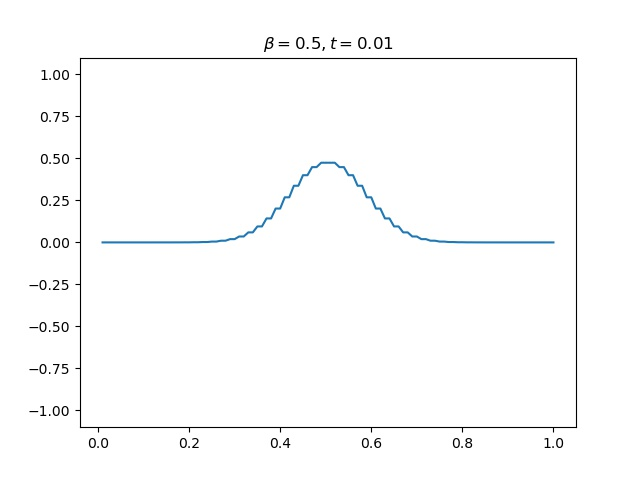
\includegraphics[width=5.5cm]{img/explicit/0.5-0.01/2.jpg}
}
\quad
\subfigure[t=0.03]{
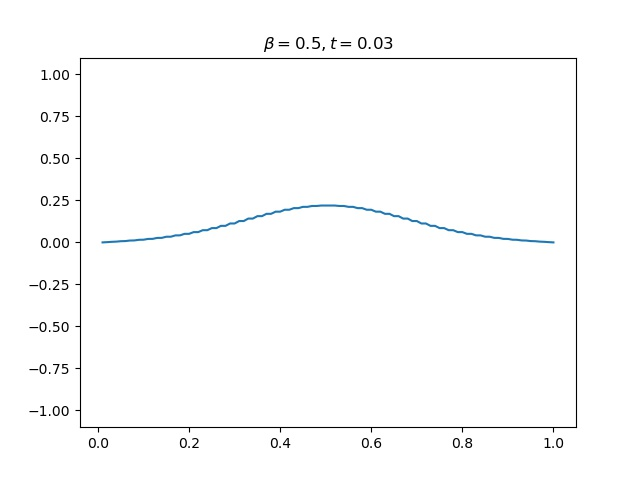
\includegraphics[width=5.5cm]{img/explicit/0.5-0.01/3.jpg}
}
\quad
\subfigure[t=0.20]{
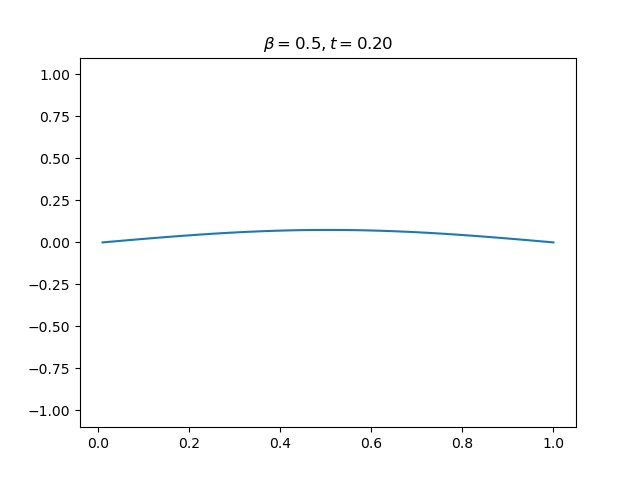
\includegraphics[width=5.5cm]{img/explicit/0.5-0.01/4.jpg}
}
\caption{显式差分,$\Delta x = 0.01,\Delta t = 0.0001,\beta = 0.5$}
\end{figure}
\begin{figure}[H]
\centering
\subfigure[t=0]{
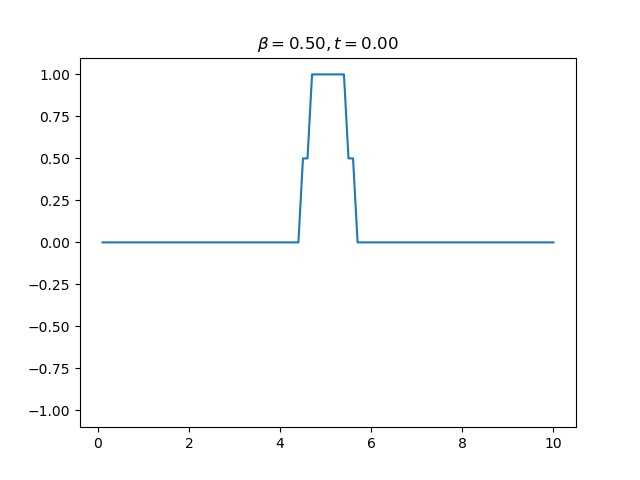
\includegraphics[width=5.5cm]{img/explicit/0.5-0.1/1.jpg}
%\caption{fig1}
}
\quad
\subfigure[t=0.20]{
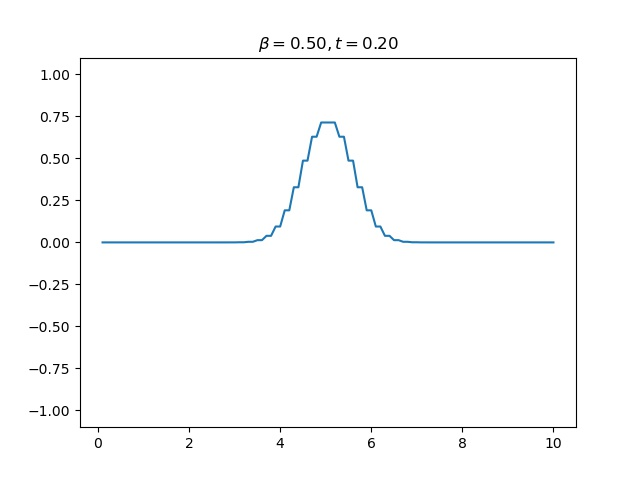
\includegraphics[width=5.5cm]{img/explicit/0.5-0.1/2.jpg}
}
\quad
\subfigure[t=2.10]{
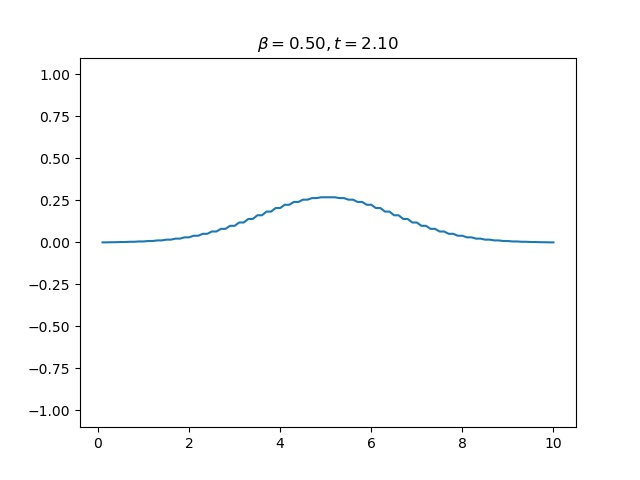
\includegraphics[width=5.5cm]{img/explicit/0.5-0.1/3.jpg}
}
\quad
\subfigure[t=9.90]{
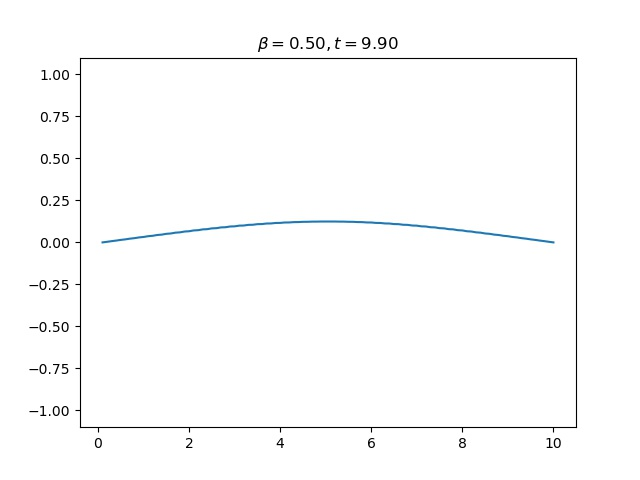
\includegraphics[width=5.5cm]{img/explicit/0.5-0.1/4.jpg}
}
\caption{显式差分,$\Delta x = 0.1,\Delta t = 0.01,\beta = 0.5$}
\end{figure}
接下来,我们稍微改变一点点$\Delta t$值,使得$\beta$值略大于0.5,可以发现,此时,差分格式立刻变得不稳定了(见图3,图4).扩散行为表现出奇异现象,并且数值急剧增大,并最终溢出.\\
\begin{figure}[H]
\centering
\subfigure[t=0]{
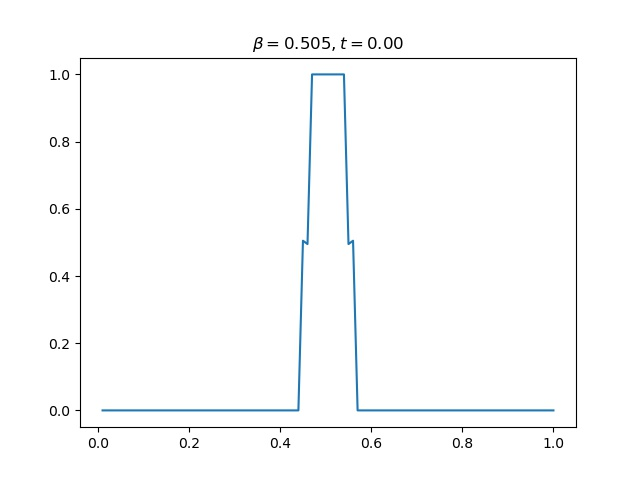
\includegraphics[width=5.5cm]{img/implicit/0.505-0.01/1.jpg}
%\caption{fig1}
}
\quad
\subfigure[t=0.20]{
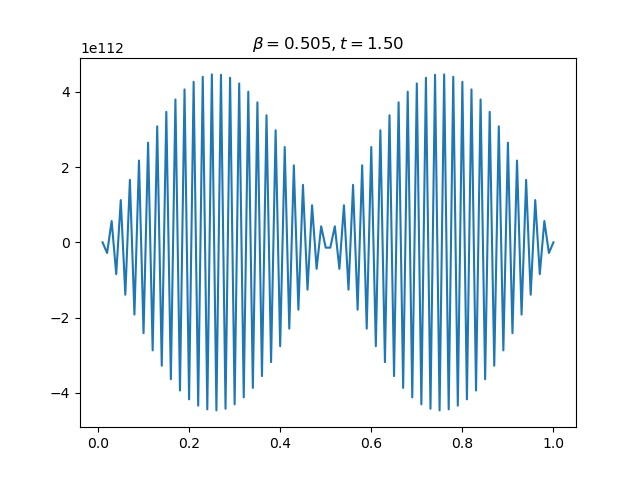
\includegraphics[width=5.5cm]{img/implicit/0.505-0.01/2.jpg}
}
\quad
\subfigure[t=1.50]{
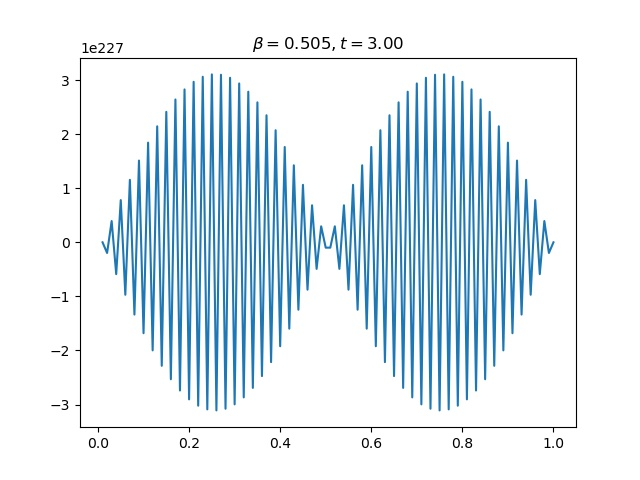
\includegraphics[width=5.5cm]{img/implicit/0.505-0.01/3.jpg}
}
\quad
\subfigure[t=4.00]{
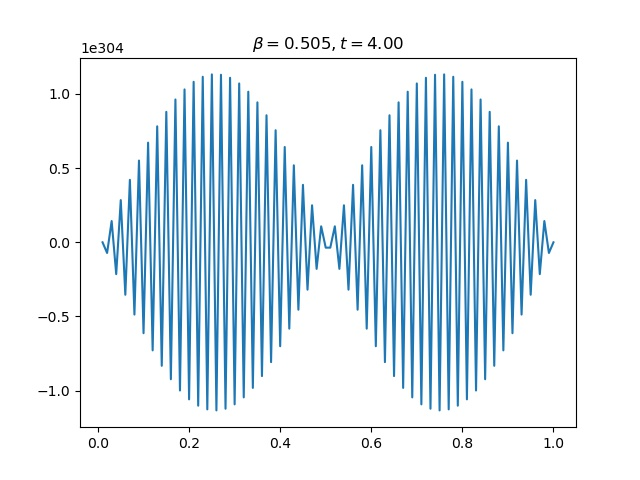
\includegraphics[width=5.5cm]{img/implicit/0.505-0.01/4.jpg}
}
\caption{显式差分,$\Delta x = 0.01,\Delta t = 0.000101,\beta = 0.505$}
\end{figure}
\begin{figure}[H]
\centering
\subfigure[t=0]{
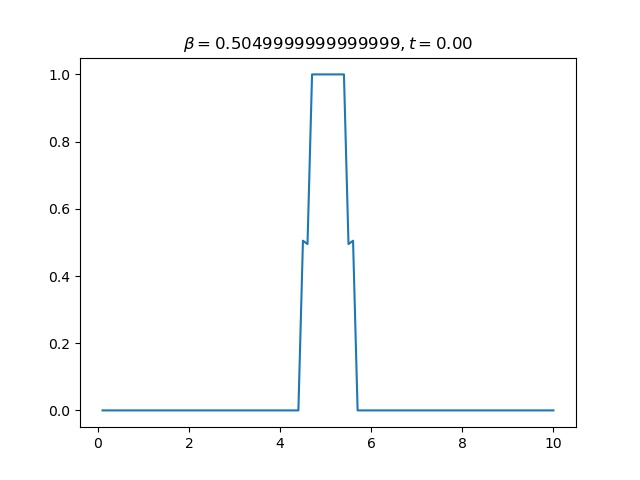
\includegraphics[width=5.5cm]{img/implicit/0.505-0.1/1.jpg}
%\caption{fig1}
}
\quad
\subfigure[t=150]{
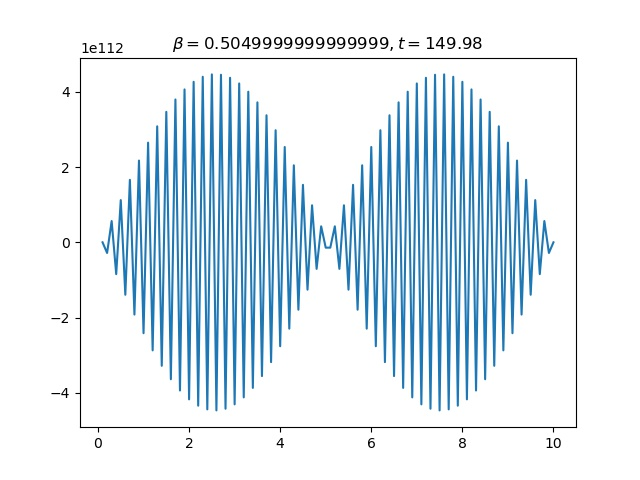
\includegraphics[width=5.5cm]{img/implicit/0.505-0.1/2.jpg}
}
\quad
\subfigure[t=300]{
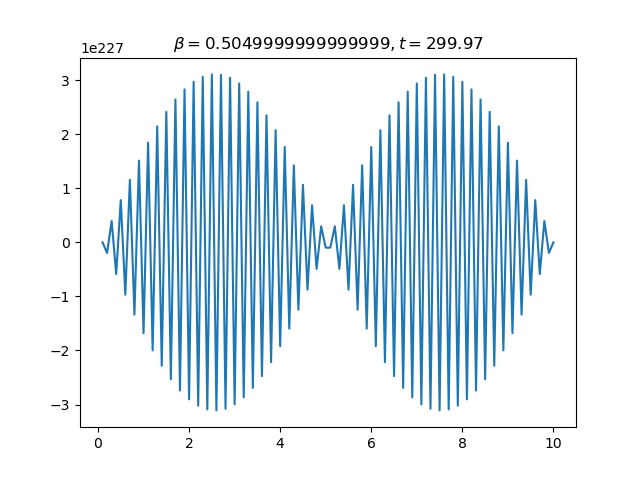
\includegraphics[width=5.5cm]{img/implicit/0.505-0.1/3.jpg}
}
\quad
\subfigure[t=390]{
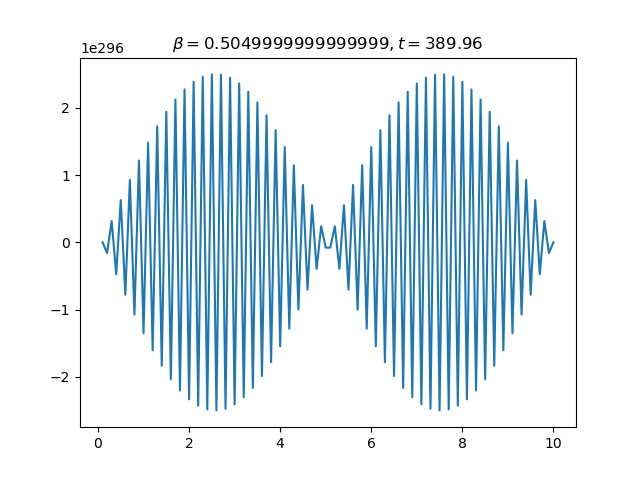
\includegraphics[width=5.5cm]{img/implicit/0.505-0.1/4.jpg}
}
\caption{显式差分,$\Delta x = 0.01,\Delta t = 0.000101,\beta = 0.505$}
\end{figure}
\subsection{隐式格式差分}
下面我来介绍隐式格式差分.差分方程如下:
\begin{equation}
     \frac{u^{n+1}_j - u^n_j}{\Delta t} = \alpha\frac{u^{n+1}_{j+1}-2u^{n+1}_j + u^{n+1}_{j-1}}{(\Delta x)^2}
\end{equation}
转化可得:
\begin{equation}
    u^{n+1}_j - \frac{\alpha\Delta t}{(\Delta x)^2}(u^{n+1}_{j+1}+u^{n+1}_{j-1}-2u^{n+1}_j) = u^n_j
\end{equation}
表面上看起来,左侧包含多个$n+1$时刻的值,难以求解,实际上,将左侧写成矩阵的形式:
\begin{equation}
A\textbf{u}^{n+1} = \textbf{u}^n\qquad A = 1-\frac{\alpha\Delta t}{(\Delta x)^2}M
\end{equation}
其中M为:
$$M = \begin{pmatrix}
-2&1&0&0&\cdots&0\\
1&-2&1&0&\cdots&0\\
0&1&-2&1&\cdots&0\\
\vdots& & & & &\vdots\\
0&0&0&0&\cdots&-2
\end{pmatrix}$$
由此,我们可以看出,只要求的矩阵A的逆,就能由$\textbf{u}^n$求得$\textbf{u}^{n+1}$:
\begin{equation}
    \mathbf{u}^{n+1} = A^{-1}\mathbf{u}^n
\end{equation}
讨论完隐式格式差分的求解,我们来看看隐式格式差分的稳定性.明显的,差分格式的误差迭代系数$G$具有和(3.1.5)一样的形式:
\begin{equation}
    G = e^{a\Delta t}
\end{equation}
同样的,对差分方程的分析将给出类似于(3.1.6)的结果,除了方程右侧是$n+1$时刻的迭代值,因此含有一个$e^{a\Delta t}$因子:
\begin{equation}
    e^{a\Delta t} = 1+\frac{\alpha \Delta t}{(\Delta x)^2}e^{a\Delta t}\left(e^{i k_{m} \Delta x}+e^{-i k_{m} \Delta x}-2\right)
\end{equation}
重排:
\begin{equation}
    e^{a\Delta t} = \left(1-\frac{\alpha\Delta t}{(\Delta x)^2}\left(e^{i k_{m} \Delta x}+e^{-i k_{m} \Delta x}-2\right)\right)^{-1}
\end{equation}
差分格式的稳定性要求:
\begin{equation}
    |G| = |e^{a\Delta t}|\leq 1
\end{equation}
同时代入Euler方程,得:
\begin{equation}
    1+\frac{4 \alpha \Delta t}{\Delta x^{2}} \sin ^{2}\left(k_{m} \Delta x / 2\right)\geq 1
\end{equation}
明显的,由于$\alpha>0,\sin ^{2}\left(k_{m} \Delta x / 2\right)>0$,(3.2.9)对于任何$\Delta t,\Delta x$的组合均成立,即意味着,隐式格式差分的稳定性不依赖于网格参数的选择.\\
我实现了隐式格式差分计算(代码见附录代码2),并计算了两组不同的$\Delta x-\Delta t$值的组合下体系的行为.结果如图5,图6所示.可以看出,即使体系的$\beta$远大于显示格式差分的稳定阈值(我们最大测试了$beta=50$的情况,此时时间步长为$\Delta t = 1s$),体系仍然能够保持稳定.这也验证了我的预测.
\begin{figure}[H]
\centering
\subfigure[t=0]{
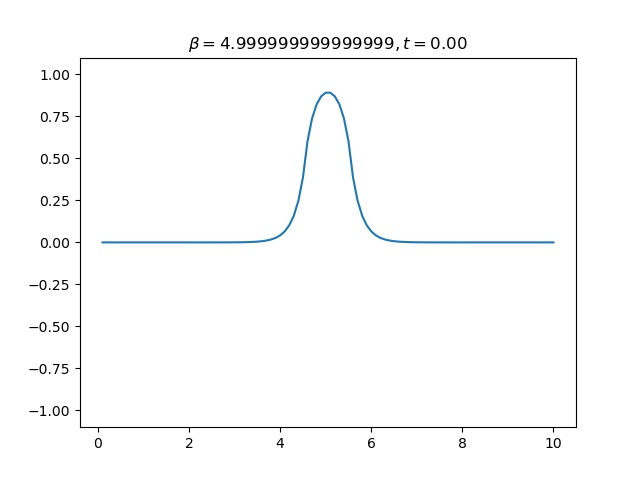
\includegraphics[width=5.5cm]{img/fig/5/1.jpg}
%\caption{fig1}
}
\quad
\subfigure[t=0.3]{
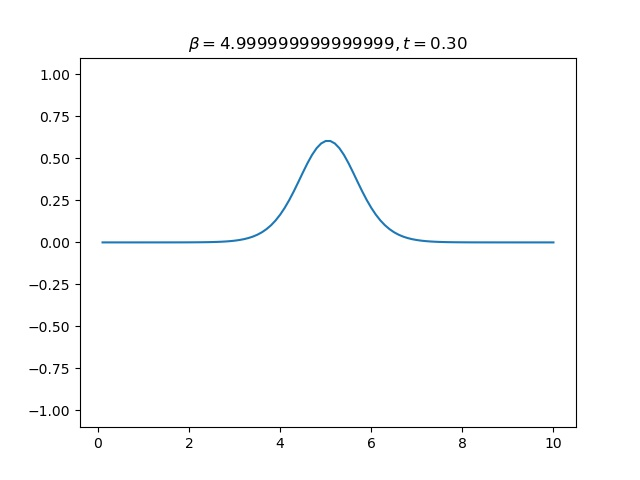
\includegraphics[width=5.5cm]{img/fig/5/2.jpg}
}
\quad
\subfigure[t=1.6]{
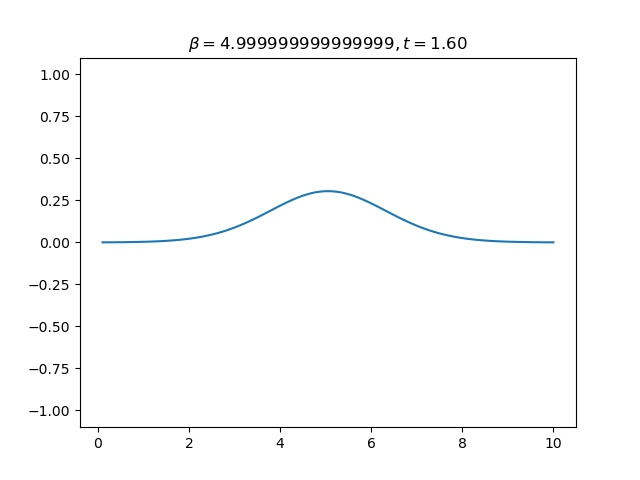
\includegraphics[width=5.5cm]{img/fig/5/3.jpg}
}
\quad
\subfigure[t=9.9]{
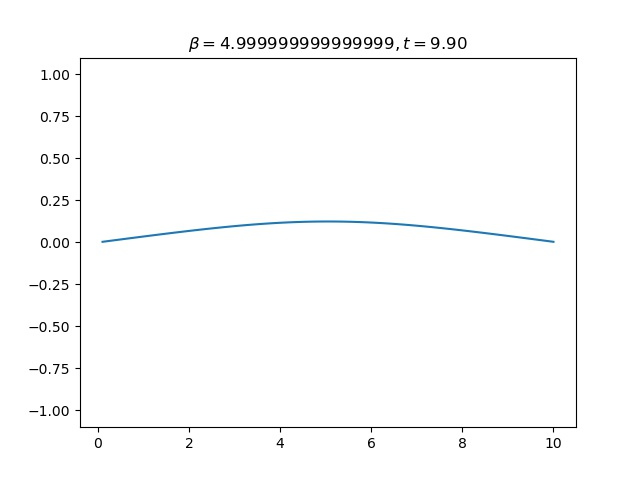
\includegraphics[width=5.5cm]{img/fig/5/4.jpg}
}
\caption{隐式差分,$\Delta x = 0.1,\Delta t = 0.1,\beta = 5$}
\end{figure}
\begin{figure}[H]
\centering
\subfigure[t=0]{
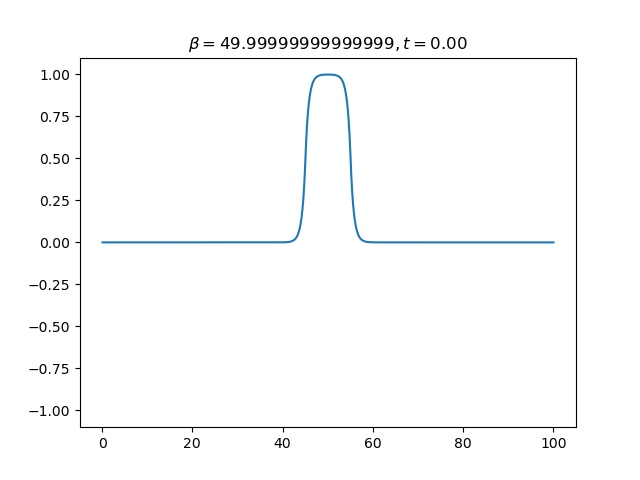
\includegraphics[width=5.5cm]{img/fig/50/1.jpg}
%\caption{fig1}
}
\quad
\subfigure[t=40]{
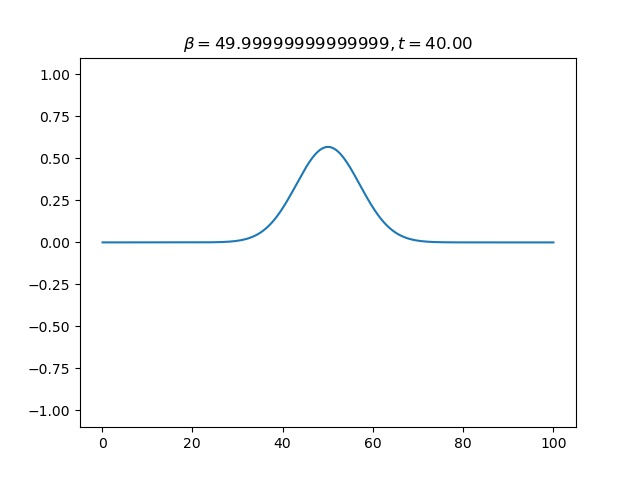
\includegraphics[width=5.5cm]{img/fig/50/2.jpg}
}
\quad
\subfigure[t=150]{
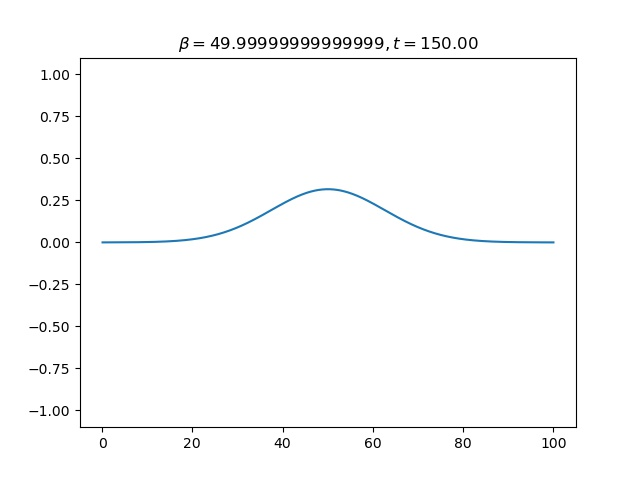
\includegraphics[width=5.5cm]{img/fig/50/3.jpg}
}
\quad
\subfigure[t=990]{
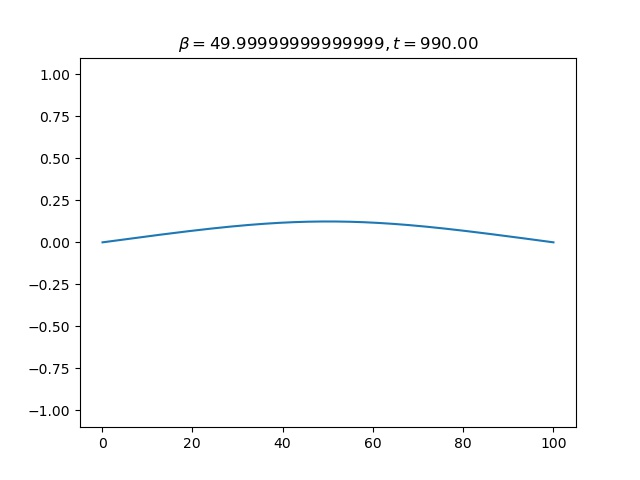
\includegraphics[width=5.5cm]{img/fig/50/4.jpg}
}
\caption{隐式差分,$\Delta x = 0.1,\Delta t = 1,\beta = 50$}
\end{figure}

\section{总结}
本文中,我介绍了分析PDE的有限差分法的稳定性的方法,并以一维扩散方程为例,分别计算了显式和隐式差分方程的稳定性条件.结果表明,对于显式方程,随着空间网格的减小,时间步长也必须随着减小,二者之间关系必须满足(3.1.9)式,否则计算误差将会发散.而对于隐式方程,则是无条件稳定的.我也使用代码分别计算了几种情况下算法的稳定性,结果与理论预测一致.
\section{附录}
\lstinputlisting[
    style       =   Python,
    caption     =   {显式形式求解},
    label       =   {Explicit.py}
]{code/explicit.py}
\lstinputlisting[
    style       =   Python,
    caption     =   {隐式形式求解},
    label       =   {Implicit.py}
]{code/implicit.py}
\clearpage
\small{
\bibliographystyle{ieee.bst}
\bibliography{reference.bib}
}
\end{document}
